% thesis.tex
% Jeremy Barnes, 1999
% $Id$

\documentclass[a4paper,11pt,oneside]{book}

\usepackage{graphics}
\usepackage{amsmath}
\usepackage{amsfonts}
\usepackage{amssymb}

% Times new roman font: smaller so less pages
%\usepackage{times}

% Get a decent page width
\oddsidemargin 0.1 in      %   Left margin on odd-numbered pages.
\evensidemargin 0.15 in    %   Left margin on even-numbered pages.
\marginparwidth 1 in       %   Width of marginal notes.
\oddsidemargin 0.125 in    %   Note that \oddsidemargin = \evensidemargin
\evensidemargin 0.125 in
\marginparwidth 0.75 in
\textwidth 6.125 in % Width of text line.

\title{Capacity Control in Boosting using a $p$-Convex Hull}
\author{Jeremy Peter Barnes}

\titlepage

\begin{document}

\frontmatter

\maketitle
\tableofcontents
\listoffigures
\listoftables

% According to the thesis rules, spacing must be at least 1.2 times normal
\renewcommand{\baselinestretch}{1.2}

% abstract.tex
% Jeremy Barnes, 1999
% $Id$

\chapter{Abstract}

A machine learning algorithm attempts to infer a general relationship
from a limited number of observations of a process.  Boosting
algorithms are a class of machine learning algorithms that improve the
performance of a so-called ``weak'' machine learning algorithm by
combining many ``weak'' hypotheses in a \emph{combined hypothesis}.
This combined hypothesis is constructed in a manner that forces
difficult-to-learn examples to be emphasised in the learning process.
The first such boosting algorithm was called ``AdaBoost''.

The performance of boosting algorithms is good to exceptional,
especially on low-noise data.  However it has recently been observed
that boosting algorithms overfit (fit the measurement noise of the
observations rather than the underlying data) on datasets containing
noisy observations, which degrades the performance.  One way of
avoiding overfitting is to limit the complexity of the combined
hypothesis (conceptually, impose a smoothness constraint) so that it
is not possible for the boosting algorithm to generate an overfitted
hypothesis.  This process is known as \emph{capacity control}.

We consider a modification to the boosting algorithm to allow the
capacity to be explicitly controlled via a $p$ parameter.  The details
of the implementation involve constraining the boosting algorithm to
generate only hypotheses that lie within a $p$-convex combination of
the weak hypotheses.  Several alternative algorithms based upon this
idea are developed; these are collectively called ``$p$-boosting
algorithms''.

A number of simulations were performed, which indicate that the best
of these algorithms outperforms AdaBoost by a modest amount (at best
18\% test error vs 25\%) on low-dimensional, noisy datasets (at the
cost of significantly increased training time).  The generalisation
ability over other datasets was not significantly different from
AdaBoost; more extensive testing is required to draw firm conclusions
on the merit of these $p$-boosting algorithms.

The $p$-convex hull approach is complementary to other AdaBoost
variants also designed to improve performance on noisy datasets (soft
margins \cite{Ratsch98}, DOOM I/II \cite{Mason99}), allowing the
possibility a combined approach superior to either.


% acknowledgements.tex
% Jeremy Barnes, 21/9/1999
% $Id$

\chapter{Acknowledgements}

Peter Bartlett
Gunnar Raetsch (proper spelling?)



\mainmatter

% intro.tex
% Jeremy Barnes, 21/9/1999
% $Id$

\chapter{Introduction}

This thesis is an investigation of a method of
overcoming a known problem (\emph{overfitting}) of a particular
machine learning algorithm (the \emph{Boosting} algorithm).  The
result is a series of machine learning algorithms called
\emph{$p$-boosting algorithms}.  These algorithms are developed,
analysed and tested in the later part of this thesis.


\section{Overview}

This introduction provides an overview of the rest of the thesis, and
covers the bigger picture, describing the field of machine learning
and its applications to practical problems.  The rest of the thesis is
composed of four parts.

\subsection*{Part I: Background}

The next few chapters rapidly narrow the focus.  Chapter
\ref{chapter:slt} describes the field of \emph{Statistical learning
theory} (SLT)\footnote{A table of acronyms is provided in appendix
\ref{appendix:acronyms}}, which provides much of the theoretical
foundations of, but does not encompass, the entire field of machine
learning.  Assumptions of \emph{binary problems} and
\emph{classification problems} also further restrict the scope of the
investigation.

Chapter \ref{chapter:stumps} provides a description of, and proves
some properties of, a very simple learning algorithm called
\emph{decision stumps} which fits within this restricted scope imposed
by the assumptions in the first two chapters.  This learning algorithm
is used as a base for the more powerful Boosting algorithms described
later.

With the necessary background in place, the \emph{Boosting} algorithm
is described in chapter \ref{chapter:boosting}.  This algorithm forms
the starting point for the original work that is considered in further
chapters.  A formal definition of what it means for an algorithm to
``boost'' is given, and many properties of the Boosting algorithm are
given.  Finally the problem of overfitting in boosting is
investigatied, as a prelude to the possible solutions investigated
throughout the remainder of the thesis.

\subsection*{Part 2: Theoretical investigation}

The key inventive step of the work described in this thesis is the use of a
\emph{$p$-convex hull} to reduce the problem of overfitting.  Chapter
\ref{chapter:pboosting} investigates the theoretical justification
behind this line of reasoning in some detail.

Chapter \ref{chapter:development} develops these abstract ideas into
concrete algorithms, and describes some properties of these
algorithms.

\subsection*{Part 3: Testing}

Chapter \ref{chapter:method} describes how these algorithms were
tested.  Chapter \ref{chapter:results} details the results of the
investigations.

\subsection*{Part 4: Discussions}

The chapters in this part evaluate the project.  (I'll fill this in
when I've done it...)


\section{The scheme of things}

This section provides an overview of the context in which this project
exists, starting very broadly and rapidly focusing on the immediate
background.


\subsection{Artificial intelligence}

The broadest possible subject area in which this work is contained is
often described as \emph{artificial intelligence}.  This field
essentially contains our efforts to make computers act in a similar
manner to humans.

This field encompasses a large body of history, philosophy and
knowledge (see, for example \cite{Penrose89}).  We will ignore much
of this, and concentrate on efforts to make a computer ``think'' like
a human.

Early work in this field (from the 1950s to the 1980s) was based on
the idea that intelligence can be emulated with a large set of rules.
The systems generated as a result, known as \emph{expert systems},
were huge databases of human-generated rules that were meant to
represent the complete knowledge of a human expert on a particular
domain.  These systems were reasonably successful at first, but became
unwieldy as the number of rules increased (a large amount of effort is
required to generate even the 1000 rules that were used in large
expert systems in 1980). 

The problem was more practical than theoretical: systems with large
numbers of rules can theoretically learn any learnable problem; it is
\emph{generating} the rules that is hard.  The next step, obvious in
hindsight, was to invent machines that could generate their own
rules; machines that could \emph{learn}.


\subsection{Machine learning}

These machines came in two flavours.  \emph{Supervised learners} are
shown examples of some kind of relationship, along with the ``right''
answers (from some form of supervisor) and attempt to learn a
relationship such that their answer always matches that of the
supervisor.  An example is trying to learn who is likely to default on
loan payments from the credit history of previous customers (the
``supervisor'' is simply the information on whether the previous
customer defaulted on their loan).  All algorithms discussed in the
body of this thesis are supervised algorithms.

\emph{Unsupervised learners} are given a set of data and asked to
learn a pattern in the data (for example, identifying interesting
clumps of stars from telescope images).


\subsection{Statistical learning theory}

Statistical learning theory provides the theoretical foundation upon
which machine learning rests.  It provides a body of knowledge that
allows bounds on the performance of learning algorithms to be
generated.  Much of this theory can be attributed to V.M.Vapnik
\ref{Vapnik95}.

Results from statistical learning theory enable us to design learning
machines which we can be sure will learn a function that is close to
the optimal.

\subsection{Voting methods}

Boosting and $p$-boosting are both examples of \emph{voting methods},
a relatively new class of algorithms which operate in a bootstrap-like
manner by combining many ``weak'' algorithms to generate a composite
algorithm.  The success of these algorithms has been remarkable; to
such an extent that the focus of machine learning research has in
recent years shifted away from the classical algorithms (all of which
are more or less equal when boosted) and on to developments in voting
methods.

These algorithms were initially thought to be immune to many of the
problems of overfitting.  Recent research has indicated that this is
not the case, however.

\section{Overfitting}

Overfitting, simply put, is learning the specifics of a process too
well to be able to apply the knowledge to a more general problem.
A familiar example for many people would be driving a familiar route
on ``auto-pilot'' and almost coming to grief on a new obstacle.

Statistical learning theory gives us a theoretical reason for
overfitting, and also an insight into how it may be avoided.  


\section{Original work}

The original work of this thesis is motivated by observations of a
theoretical bound on overfitting; and in particular on a method of
reducing overfitting in the boosting algorithm.  This theory is first
developed into several practical algorithms; these algorithms are then
tested against the original AdaBoost algorithm and for compliance with
the theory behind them.





\part{Background}
% slt.tex
% Jeremy Barnes, 1999
% $Id$

\chapter{Statistical learning theory}
\label{chapter:slt}


\section{Formulation of machine learning}

We first develop some conventions and notation.

\subsection{Learning machines}
A \emph{learning method} (or what we will call here a \emph{learning
machine} is described in Cherkassky and Mulier \cite{Cherkassky98} as
%
\begin{quote}
	\ldots an algorithm (usually implemented in software) that
	estimates an unknown mapping (dependency) between a system's
	inputs and outputs from the available data, namely from known
	(input, output) samples.
\end{quote}
%
This motivates the formal definition of supervised learning,
which is illustrated in figure \ref{fig:supervised learning}.  The generator
produces samples $\mathbf{x}$ drawn from a fixed (but unknown)
probability distribution $p(x)$\footnote{In practice, these samples
are normally \emph{observed} rather then \emph{generated}.}.
These samples are presented both to
a supervisor (which produces the ``correct'' result $\mathbf{y}$) and to the
learning machine (which produces its estimate $\hat{\mathbf{y}}$).  The
learning machine can use the difference between these two results
($\bfyh - \bfy$) as feedback to improve its approximation.  The goal
is for the learning machine to always generate the correct
estimate, such that $\mathbf{\hat{y} - y = 0}$ for all samples $\mathbf{x}$.

\begin{linefigure}
\begin{center}
\begin{picture}(270,155)(30,20)
\put(30,110){\framebox(60, 60){\parbox{55pt}{\center{Sample generator}}}}
\put(150,110){\framebox(60, 60){\parbox{55pt}{\center{Learning machine
$\hat{h}(\mathbf{x})$}}}}
\put(150,30){\framebox(60, 40){\parbox{55pt}{\center{Supervisor
$h(\mathbf{x})$}}}}
\put(90, 140){\vector(1,0){60}}
\put(120,140){\line(0,-1){90}}
\put(120,50){\vector(1,0){30}}
\put(120,150){\framebox(0,0){$\mathbf{x}$}}
\put(210,50){\line(1,0){30}}
\put(240,130){\line(0,-1){80}}
\put(250,90){\framebox(0,0){$\mathbf{y}$}}
\put(240,130){\vector(-1,0){30}}
\put(210,150){\vector(1,0){60}}
\put(280,150){\framebox(0,0){$\hat{\mathbf{y}}$}}
\end{picture}
\end{center}
\caption{Supervised learning}
\label{fig:supervised learning}
\end{linefigure}

\subsubsection{Sample generator}
\label{sec:sample generator}

The sample generator drives the learning process, by generating a
series of samples $\mathbf{x}_1, \ldots$ for the learning machine to
operate on.  Each $\mathbf{x}_i \in \mathcal{I}$ where $\mathcal{I}$
is the ``input space'', and $\mathcal{I} \subseteq \mathbb{R}^n$ where
$n$ is the dimensionality of the sample space.


\subsubsection{Supervisor}
\label{sec:supervisor}

The supervisor is a function
%
\begin{equation}
\mathbf{y} = h(\mathbf{x}) \qquad \mbox{where} \qquad \mathbf{x} \in
\mathcal{I} \qquad \mbox{and} \qquad \mathbf{y} \in \mathcal{O}
\label{eqn:supervisor}
\end{equation}
%
that always generates the ``correct'' answer given an input $\mathbf{x}$.

There is potential for confusion concerning the word ``correct'' in
the previous statement.  The correct answer or distribution is
usually not known, and the data observed from it may be noisy.  This
noisy data, while usually containing errors, is still termed the
correct data.


\subsubsection{Learning machine}
\label{sec:learning machine}

The learning machine is a function operating on the same domain and
range as the supervisor:
%
\begin{equation}
\mathbf{\hat{y}} = \hat{h}(\mathbf{x}) \qquad \mbox{where} \qquad
\mathbf{x} \in \mathcal{I} \qquad \mbox{and} \qquad \mathbf{y} \in
\mathcal{O}
\label{eqn:learning machine formulation}
\end{equation}
%
Any useful learning machine exhibits a learning behaviour (not shown in
equation \ref{eqn:learning machine formulation}, whereby the function
$\hat{h}(\cdot)$ is updated based on the error feedback
$\mathbf{\hat{y} - y = 0}$.


\subsection{Domain and range of learning machines}

The input set \calI\ and output set \calO\ specify the domain and
range of the learning problem.  The input set depends upon number and
range of input variables in the problem; in the datasets considered in
this thesis, usually $\mathcal{I} = [0,1] \times [0,1] \subset
\mathbb{R}^2$.

The ``output set'' $\mathcal{O}$ is defined as $\mathcal{I} \subseteq
\mathbb{R}^m$ where $m$ is the dimensionality of the output space (or
the number of output variables).

In almost all cases, there is only one output variable ($m=1$) or the
multiple output variables are independent and can each
be generated by a separate learning machine with $m=1$.
Thus it is reasonable to restrict our attention to the case where
$m=1$ for the rest of this thesis.

The distinction between \emph{classification} and \emph{regression}
problems is made on the size of $\mathcal{O}$.


\subsubsection{Regression}
\label{sec:regression}

A learning machine is solving a regression problem when the size of
the output space $\|\mathcal{O}\|$ is infinite.  Usually, this means
that $\mathcal{O}$ is some interval on $\mathbb{R}$.  This thesis does
not consider regression problems (although it may not be difficult to 
generalise some of the results to include regression problems); thus
regression is not considered further.


\subsubsection{Classification}
\label{sec:classification}

Whenever $\|\calO\| < \infty$ we are solving a classification
problem.  (Learning machines which solve a classification problem are
often called \emph{classifiers}).

Our permissible $y$ values are now a finite number of discrete values
(\emph{categories}): 
%
\begin{equation}
\mathcal{I} = \{y_1, y_2, \ldots, y_c\}, \qquad \mbox{where} \qquad y_1, y_2,
\ldots, y_c \in \mathbb{R}^m
\end{equation}
%
A sample classification problem is shown in
figure \ref{fig:classification problem}.

A classification problem involves splitting the input space
into a set of disjoint regions $\{ \mathcal{R}_1 \ldots \mathcal{R}_c
\}$ which correspond to the category values.  A useful representation
of these regions is gained by constructing the ``decision boundaries''
as illustrated in figure \ref{fig:classification problem}.

\begin{linefigure}
\begin{center}
\includegraphics{figures/classification_problem.epsg}
\end{center}
\caption{A classification problem}
\label{fig:classification problem}
The $\times$ symbol represents $y=-1$ and the $\circ$ symbol $y=1$.
The dotted line is the ``decision boundary'', which is the boundary of
adjacent regions of different symbols.  Note that in the data shown,
there are many possible decision boundaries which classify the data
correctly.
\end{linefigure}

For the remainder of this thesis, only classification problems will be
considered.  In most cases, these will also be \emph{binary}
classification problems (two categories) where $\mathcal{O} = \{-1,
1\}$.

\subsection{Alternative formulation for binary classification problems}

The discontinuities in the output of a classifier tend to make
analysis difficult.  The formulation developed in this section
alleviates much of this difficulty by defining the output of a
classifier as the  \emph{sign of a real valued function}.  This real
valued function in known as the \emph{margin}.

We recast (\ref{eqn:learning machine formulation}) in the form
%
\begin{equation}
y = \sign \left( f(\mathbf{x}) \right)
\label{eqn:marginal classification formulation}
\end{equation}
%
where the margin function $f : \mathbb{R}^n \mapsto \mathbb{R}$ and
%
\begin{equation}
\sign (x) = \left\{ \begin{array}{rl}
1	& \qquad \mbox{if $x \geq 0$} \\
-1	& \qquad \mbox{otherwise}
\end{array} \right.
\end{equation}
%

Putting these together explicitly, we find
%
\begin{equation}
m_{\mathbf{x}} = \left\{ \begin{array}{rl}
yf(\mathbf{x})	& \qquad \mbox{if $y = \hat{y}$} \\
-yf(\mathbf{x})	& \qquad \mbox{if $y \neq \hat{y}$}
\end{array} \right.
\label{eqn:margin definition}
\end{equation}

The magnitude of the margin at a point is an indication of how sure the
learning machine is of its classification.  Geometrically, for
``nicely behaved'' functions the distance between a point and the
decision boundary will roughly correspond to the magnitude of the
margin at that point.  See figure \ref{fig:margin illustration} for an
illustration of this. 

\begin{linefigure}
\begin{center}
\includegraphics{figures/margin_illustration.epsg}
\end{center}
\caption{The margin of a sample}
\emph{The dotted line denotes the decision boundary and the $\times$ the
point for which we wish to define a margin.}
\label{fig:margin illustration}
\end{linefigure}

\subsection{Summary}

In this section we have defined the classification problem and much of
the notation used to describe it.  We also introduced the concept of
the margin, which useful for analysing binary classification problems.



\section{Comparing and selecting learning machines: ERM}
\label{sec:erm}

Now that we have defined what we mean by a ``learning machine'' (and
in particular, what we mean by a ``classifier''), we need a way of
comparing two classifiers to determine which is ``better''.


\subsection{Loss functions}

One metric that can be used is known as a ``loss function''.  The
input to a loss function is a triple
$(\bfx, \bfyh, \bfy)$ where \bfx\ is a sample, \bfyh\ is the
output of the classifier (learning machine), and \bfy\ is the correct output (that generated by the supervisor).  See figure \ref{fig:supervised
learning}.  The output of the loss function is a single number $q$
which describes how ``bad'' this estimate is.  In symbols, the loss
function is
%
\begin{equation}
q = Q(\bfx, \bfyh, \bfy) \qquad \mbox{where} \qquad q \in \mathbb{R};
\bfx \in \calI; \mbox{ and }\bfyh, \bfy \in \calO
\end{equation}
%

In this thesis, only one loss function will be considered.  This is
known as the ``misclassification loss function'', and is defined as
%
\begin{equation}
Q(\bfx, \bfyh, \bfy) = Q(\bfyh, \bfy) = \left\{
\begin{array}{ll}
	0	&	\qquad \mbox{if $\bfyh = \bfy$} \\
	1	&	\qquad \mbox{if $\bfyh \neq \bfy$}
\end{array}
\right.
\label{eqn:misclassification loss function}
\end{equation}
%
which does \emph{not} depend upon the position in the input space \bfx.

This loss function is very easy to understand: given a series of input
samples, the sum of the loss functions will be equal to the number of
samples that were misclassified.  If the performance of two
classifiers are compared using this loss function, then the one with
the lowest risk will be the one that makes the least ``mistakes''.


\subsection{True risk}
Given our loss function $Q(\cdot)$, we are now in the position to be
able to compare the performance of a number of classifiers over the
entire input space.  We define the \emph{true risk} of a classifier
$\hat{h}(\bfx)$ given a supervisor $h(\bfx)$ as
%
\begin{equation}
R(\hat{h}) = \int_{\calI} Q(\bfx, \bfyh, \bfy) \: p(\bfx) \: d\bfx
\label{eqn:true risk}
\end{equation}
%
where $p(\bfx)$ is the marginal probability that sample $\bfx$ will be
generated.

Using our loss function \ref{eqn:misclassification loss function}, the
value of $R$ is easily seem to be the proportion of samples that are
misclassified.

The goal of machine learning theory is generate learning
machines that minimise the true risk \ref{eqn:true risk}.
Unfortunately, this is impossible:
%
\begin{enumerate}
\item	Generally, \ref{eqn:true risk} cannot be solved analytically,
	or in finite time, making the minimisation of it impossible.
%
\item	In practice, there are only a finite number of observations
	$(\bfx_1, \bfy_1), \ldots, (\bfx_l, \bfy_l)$ available.  Thus
	it is impossible to evaluate \ref{eqn:true risk}.
\end{enumerate}
%
We use something that is the best we can calculate: the
\emph{empirical risk}.


\subsection{Empirical risk}
Empirical risk is a weaker version of true risk, that can be
evaluated.  Given a set of $l$ observations
$\{(\bfx_1, \bfy_1), \ldots, (\bfx_l, \bfy_l)\}$ and setting $\bfyh_i
= \hat{h}(\bfy_i)$ as the output of our learning machine $h(\cdot)$,
we can define our empirical risk as 
%
\begin{equation}
R_{\emp} = \frac{1}{l} \sum_{i=1}^{l} Q(\bfx_i, \bfy_i, \bfyh_i)
\end{equation}
%
The following observations concern the empirical risk:
%
\begin{itemize}
\item 	As $l \rightarrow \infty$, and assuming that $\bfx$ is evenly
	distributed over \calI\, (and that $Q$ is reasonably well
	behaved), we would expect that $R_{\emp}(\cdot) \rightarrow
	R(\cdot)$.

\item	$R_{\emp}$ is the ``best that we can do'', in that it uses all
	available observations.  However, there is further scope for
	\emph{a priori} knowledge of the system to be used via the
	selection of an appropriate model.

\item	Section \ref{sec:slt} explores the rate of convergence of
	empirical risk $R_{\emp}$ to true risk $R$.
\end{itemize}

\subsection{Empirical risk minimisation}

We have been concerned thus far with a \emph{single} learning
machine $\hat{h}(\cdot)$.  However the goal of machine learning is to
pick the optional $\hat{h}$  from a set \calH\ of learning machines.
Given our metric of \emph{empirical risk}, we are able to define an
inductive principle that minimises the empirical risk.  This principle
is known as \emph{empirical risk minimisation} (ERM):

Assume that we have a set of learning machines
%
\begin{equation}
\hat{h}_i \in \calH \qquad \mbox{where} \qquad h_i : \calI \mapsto
\calO
\end{equation}
%
and a loss function $Q$.

Then the principle of \emph{empirical risk minimisation} selects the
optimal learning machine $\hat{h}^{\ast} \in \calH$ in the sense that
the empirical risk is minimised:
%
\begin{equation}
\hat{h}^{\ast} = \arg \min_{\hat{h} \in \calH} R_{\emp}(\hat{h})
\label{eqn:erm}
\end{equation}

\subsection{Summary}

This section considered metrics that can be used to compare different
learning machines.  The true risk is the ideal measure, but cannot be
evaluated in practice.  The empirical risk is a more pragmatic
measure.  The logical next step is the empirical risk minimisation
inductive principle, which simply chooses the learning algorithm with
the minimum empirical risk.





\section{Statistical learning theory}
\label{sec:slt}

We now have framework and an inductive principle for choosing the
best learning machine $\hat{h}_{\mbox{opt}}$ from a set $\calH$ over a
set of \emph{known training data}.  The ideas that are developed in
this section allow the performance of the learning machine to be
predicted over \emph{unknown} (test) data.  In other words, we are now
trying to measure the generalisation ability of the learning machine.

This section develops important results from statistical learning
theory (SLT).  SLT provides a mathematically rigorous
conceptual framework in which to evaluate the many empirical results.
This theory is covered in much greater detail by Vapnik
\cite{Vapnik98} and Cherkassky \& Mulier \cite{Cherkassky98}.  Results
are also taken from Bartlett et al. \cite{Bartlett98a}.

\subsection{Performance bounds}

* Show that form of bounds is training error + other term
* Quick explanation of method for finite hypothesis space: bound the
  tail of the binomial distribution.
* Details are in \cite{Bartlett98b}.


\subsection{Vapnik-Chervonenkis dimension}

The VC dimension is a measure of the complexity of a class of
hypotheses $\calH$ that turns out to be the ``right'' measure for many
problems (this is described in more detail later).

\subsubsection{Shattering}

\begin{definition}[Shattering]
Consider a set $S$ of $h$ points $x_1 \ldots x_h \in \calI$.  Then a
function class $\calH$ is said to \emph{shatter} $S$ if and only if
there exist functions $f_1, \ldots, f_n \in \calH$ such that each of
the $n = 2^h$ possible classifications of the points are produced.
\end{definition}

Figure \ref{fig:shattering} provides an example of the shattering of
points in the plane by the set of lines in the plane.  In essence, a
function class shatters a set of points if the function class is
sufficiently complex.  The definition of the VC dimension is built
upon shattering.

\begin{linefigure}
\begin{center}
\includegraphics{figures/shattering.epsg}
\end{center}
\caption{Shattering a set of points}
\label{fig:shattering}
The $\times$ symbols are points; the lines are decision boundaries.
Part (a) shows how two points can be shattered by linear decision
boundaries.  Part (b) shows that there are no three nonincident points
cannot be shattered by a linear decision boundary.
\end{linefigure}


\subsubsection{VC dimension}

\begin{definition}[VC dimension]
Given a function class $\calH$ on $\calI \mapsto \calO$, the VC
dimension of the class is defined as
%
\begin{equation}
\VCdim{\calH} = \max_{h} : \exists S = \{\bfx_1, \ldots, \bfx_h\},
i \neq j \rightarrow \bfx_i \neq \bfx_j,
\qquad \mbox{where} \qquad \mbox{\calH\ shatters $S$}
\end{equation}
\end{definition}

In other words, $\VCdim(\calH)$ is the largest number $h$ where
a set of $h$ distinct points can be selected that is shattered by
$\calH$.  Thus in figure \ref{fig:shattering}, the VC dimension of
lines in $\mathbb{R}^2$ is 2.

For an example of a VC dimension calculation, see
chapter \ref{chapter:stumps} which calculates the VC dimension of a
very simple classification algorithm.

\subsubsection{Methods of calculating $\VCdim(\calH)$}

There are many theorems on how to calculate $\VCdim(\calH)$ for
different classes of functions (it is usually difficult to do
directly).  In many cases, a useful estimate for conceptual purposes
is
%
\begin{equation}
\VCdim(\calH) \approx \mbox{number of parameters in $\calH$}
\end{equation}
%
No difficult VC dimension calculations are required in this thesis;
thus these methods will not be considered further.

\subsubsection{Bounds using $\VCdim(\calH)$}

Having identified a good measure of the complexity of a hypothesis
space, we can now use this measure to bound the performance of
classifiers from this hypothesis space.

\begin{theorem}[VC upper bound (from \cite{Bartlett98a})]
Let $H$ be a class of functions mapping from a set $\calI$ to $\calO =
\{-1, 1\}$ and having VC-dimension $h$.  For any probability
distribution on $\calI \times \{-1,1\}$, with probability $1-\delta$
over $m$ random examples $\mathbf{x}$, any hypothesis $f$ in $\calH$
has generalisation error no more than
\begin{equation}
2\mathrm{Er}_{\mathbf{x}}(f) + \frac{1}{m} \left[ 4 \ln 
\left( \frac{4}{\delta} \right) + 4 h \ln \left( \frac{2 e l}{h}
\right) \right]
\end{equation}
provided $h \leq m$.
\end{theorem}

This upper bound holds for \emph{all} probability distributions.
However, in practice it seems to be very pessemistic.

\begin{theorem}[VC lower bound (from \cite{Bartlett98a})]
Let $H$ be a hypothesis space with finite VC dimension $h \geq 1$.
Then for any learning algorithm there exist distributions such that
with probability at least $\delta$ over $l$ random examples, the error
of $f$ is at least
\begin{equation}
\max \left[ \frac{h-1}{32l}, \frac{1}{l} \ln \left( \frac{1}{\delta}
\right) \right]
\end{equation}
\end{theorem}

This lower bound is an \emph{existance} bound; it shows that there
exist distributions in which the error gets very high.

The existence of these two bounds shows that the VC dimension is the
``right'' measure of complexity.  \marginpar{More...}


\subsection{Fat-shattering dimension}


The problem with the VC dimension is that it is sensitive to very
small changes to the scale.  For example, consider two hypothesis
spaces.  The first has the unit circle ($r(\theta) = 1$) as its decision
boundary, and $h = 2$.  The second is the set of all decision
boundaries where $|r(\theta) - 1| < \epsilon$, where $\epsilon$ is a
small number.  This has $h = \infty$.  However, it is obvious that as
$\epsilon$ get small enough the two are almost identical.  See figure
\ref{fig:fat-shattering}.

\begin{linefigure}
\begin{center}
\includegraphics{figures/fat_shattering.epsg}
\end{center}
\caption{Fat-shattering a set of points}
\label{fig:fat-shattering}
\end{linefigure}


For this reason, the \emph{fat-shattering dimension} is used.  It
is a scale-sensitive version of the VC dimension.

The differences between fat-shattering dimension and the VC dimension
are:
\begin{itemize}
\item	The fat-shattering dimension is defined at a scale $\gamma$;
\item	The fat-shattering dimension works on the \emph{margins} of a
	classifier (see section \ref{sec:margin}), a real-valued
	quantity, rather than the class ($\{\pm 1\}$).
\item	In order for a hypothesis class to $\gamma$-shatter a set of
	points, it is not sufficient that the points simply lie on the
	correct side of the decision boundary.  They must lie a
	substantial distance ($\gamma$) on that side.
\item	Thus, in general we have $\Fat{\gamma}(\calH) <
	\VCdim(\calH)$.
\end{itemize}

\subsubsection{Definition}

The definition of the fat-shattering dimension relies upon the
concept of $\gamma$-shattering.

\begin{definition}[$\gamma$-shattering]
Consider a set $S$ of $h$ points $x_1 \ldots x_h \in \calI$.  Then a
function class $\calH$ where $\calI \mapsto \calO$ is said to
\emph{$\gamma$-shatter} $S$ if and only if there exist functions $f_1,
\ldots, f_n \in \calH$ such that 
\begin{enumerate}
\item	each of the $n = 2^h$ possible classifications of the points
	are produced;
\end{enumerate}
\end{definition}
\marginpar{This is crap.}

Put a figure of $gamma$-shattering in here for clarity.  Use our
rather dodgy assertion before that the margin ``usually roughly
corresponds to the distance from the decision boundary'', but make
clear that we are using that dodgy assumption.

We now define the fat-shattering dimension in a similar manner to the
VC dimension:

\begin{definition}[Fat-shattering dimension at scale $\gamma$]
Given a function class $\calH$ on $\calI \mapsto \calO$, the
fat-shattering dimension of the class at scale $\gamma$ is defined as
%
\begin{equation}
\Fat{\gamma}(\calH) = \max_{h} : \exists S = \{\bfx_1, \ldots, \bfx_h\},
i \neq j \rightarrow \bfx_i \neq \bfx_j,
\qquad \mbox{where} \qquad \mbox{\calH\ $\gamma$-shatters $S$}
\end{equation}
\end{definition}


\subsubsection{Fat-shattering dimension - alternative definition}
These are copied verbatim from Bartlett et al. \cite{Bartlett98a}.

Let \calF\ be a set of real values functions.  We say that a set of
points $X$ is \emph{$\gamma$-shattered by \calF} if there are real
numbers $r_x$ indexed by $x \in X$ such that for all binary vectors
$b$ indexed by $X$, there is a function $f_b \in \calF$ satisfying
\begin{equation}
f_b(x)  \left\{
	\begin{array}{ll}
		\geq r_x + \gamma & \mbox{if $b_x = 1$} \\
		\leq r_x - \gamma & \mbox{otherwise}
	\end{array}
\right.
\end{equation}
The \emph{fat shattering dimension} $\fat_{\calF}$ of the set \calF\ is
a function from the positive real numbers to the integers which maps a
value $\gamma$ to the size of the largest $\gamma$-shattered set (if
this is finite), or infinity otherwise.


\subsubsection{Bounds using $\Fat{\lambda}(\calH)$}

See the explanation of this in \cite{Bartlett98a} pages 5-6.  This is
all copied directly from there.

\begin{theorem}[Bounds on large-margin classifiers]
Consider a class \calF\ of real-valued functions.  With probability at
least $1 - \delta$ over $l$ independently generated examples
$\mathbf{z}$, if a classifier $\sign (f) \in \sign (\calF)$ has margin
at least $\gamma$ on $\mathbf{z}$, then the error of $\sign (f)$ is no
more than
\begin{equation}
\frac{2}{l} \left[ h \log_2 \left( \frac{8 e l}{h} \right) \log_2(32l)
+ \log_2 \left( \frac{8l}{\delta} \right) \right]
\end{equation}
where $h = \fat_{\calF}(\gamma / 16)$.

Furthermore, with probability at least $1 - \delta$, every classifier
$\sign (f) \in \sign (\calF)$ has error no more than
\begin{equation}
b/l + \sqrt{\frac{2}{l} \left[ h \ln(34el/h) \log_2(578l) +
\ln(4/\delta) \right] }
\end{equation}
where $b$ is the number of labelled training examples with a margin
less than $\gamma$.
\end{theorem}



\subsection{Covering numbers}

Covering numbers are different from the VC dimension and the fat
shattering dimension in that we are only looking at the function in
the vicinity of a few points.

Given a number of points $x_1, \ldots, x_m$, and a class of functions
$\calH$, such that $\forall f \in \calH : \calI \mapsto \mathbb{R}$,
we define 
%
\begin{equation}
f_{|x} = (f(x_1), \ldots, f(x_m)) \in \mathbb{R}^m
\end{equation}
%
In other words, we are looking at the function only where we have a
sample.  Now typically, we will have $|\calH_{|x}| = \infty$.
However, we don't have to calculate $\calH$ exactly... we can make do
with an approximation.

The covering number is the size of an approximating set, such that all
points are within a distance $\epsilon$ of that set.  This is made
formal in the following statement:

\begin{definition}[Covering number]

Given a set $\calH_{|x}$ and a scale $\epsilon > 0$ we define the
covering number as
%
\begin{equation}
\cover{\calH_{|x}}{\epsilon} = \min \left\{
|\hat{\calH}| : \forall f \in \calH \exists \hat{f} \in \hat{calH}
 \qquad \mbox{where} \| f_{|x} - \hat{f}_{|x} \| < \epsilon \right\}
\end{equation}
\end{definition}

Thus, the covering number is a measure of the number of hypotheses
that are needed to get \emph{close enough} to the hypothesis class
$\calH$.


\subsubsection{Bounds using covering numbers}

Page 40 of Peter's slides.

\subsubsection{Methods of calculating}

\subsubsection{Application to $p$-convex hulls ($p < 1$)}

The theoretical motivation behind the algorithms developed in this
thesis uses the covering number of a $p$-convex hull ($\co_p(\calH)$).
This section defines a ``$p$-convex hull'' and gives a result on the covering
numbers for $p < 1$.  

At the moment, this whole section is copied pretty much verbatim from
\cite{Williamson99}.

The $p$-convex hull (strictly speaking, the $p$-absolutely convex hull) of
a set $\calH$ of functions (where $p>0$) is defined as
%
\begin{equation}
\cop (\calH) =
 \bigcup _{n \in \mathbb{N}}
\left\{
 \sum_{i=1}^{n}
 \alpha _i
f_i : f_1, \ldots, f_n \in F,
 \alpha _1, \ldots, \alpha _n \in \mathbb{\calH},
 \sum_{i=1}^{n} | a_i |^p \leq 1
\right\}
\end{equation}

Thus the $p$-convex hull is a subset of the set of all possible linear
combinations of functions of a class $F$, where the members of the
subset are those where $\sum_{i=1}^n |\alpha_i| \leq 1$.  The
following remarks concern $p$-convex hulls:
%
\begin{itemize}
\item	If $0 < p_1 \leq p_2 \leq \cdots \leq p_z \leq 1$, then
	$\cop 1 \subseteq \cop 2 \subseteq \cdots \subseteq \cop z$
	That is to say, the higher that $p$ is, the richer the set of
	functions in $\cop{F}$.
\item	In general, it is very hard to visualise the \emph{convex} hull
	of a set of functions, let alone the $p$-convex hull.  The
	convex hull is always richer than the function class.
\item	As an example (from Williamson et al. \cite{Williamson99}), the convex
	hull of the Heaviside functions on $[0, 1]$ is the set of
	functions of ``bounded variation''.\marginpar{Need a diagram}
\end{itemize}






% stumps.tex
% Jeremy Barnes, 22/9/1999
% $Id$

\providecommand{\emp}{\mathrm{emp}}
\providecommand{\calF}{\ensuremath{\mathcal{F}}}
\providecommand{\fat}{\ensuremath{\mathrm{fat}}}
\providecommand{\sign}{\ensuremath{\mathrm{sign}}}
\providecommand{\cop}{\ensuremath{\mathrm{co}_p}}
\providecommand{\co}{\ensuremath{\mathrm{co}}}
\providecommand{\bfx}{\ensuremath{\mathbf{x}}}
\providecommand{\bfy}{\ensuremath{\mathbf{y}}}
\providecommand{\bfyh}{\ensuremath{\hat{\mathbf{y}}}}
\providecommand{\calO}{\ensuremath{\mathcal{O}}}
\providecommand{\calI}{\ensuremath{\mathcal{I}}}
\providecommand{\calH}{\ensuremath{\mathcal{H}}}


\chapter{Decision Stumps}

\section{Description of Decision Stumps}

\section{Performance of Decision Stumps}



\section{Decision stumps and CART}

Both of the unboosted learning algorithms used in this thesis are
tree-based algorithms.  A tree-based algorithm splits the input space
$\calI$ into a number of disjoint regions.  Each of these regions may
again be split, and the algorithm continues in this recursive manner
until a termination condition is met.  Thus a tree structure is built
up.

\subsection{Decision stumps}

The decision stumps algorithm divides the input space into exactly two
regions, each of which is assigned a category.  The tree created is
very small, with only two nodes (hence the name ``decision
\emph{stumps}''.

\subsubsection{Classification}

An example of a decision boundary generated by a decision stumps
classifier is shown in figu


\subsubsection{Training}



The algorithm for the training of a decision stump is given below

\subsection{CART}

\subsubsection{Classification}

The CART algorithm splits its input space into 


  This is then repeated recursively to refine
the classification.

Both 

\subsubsection{Training}








% boosting.tex
% Jeremy Barnes, 29/8/1999
% $Id$

% The chapter of my thesis on Boosting

\chapter{Boosting and similar algorithms}
\label{chapter:boosting}

The name ``Boosting'' is applied to many different machine learning
algorithms, which combine many weak hypotheses to form a ``strong''
hypothesis that significantly outperforms them.

We first describe the classic algorithm \emph{AdaBoost}.  A full
description is given, along with some examples of its performance and
a discussion of why it performs so well.  We also give a formal
definition of what we mean by the term ``boosting''.

A useful viewpoint of the boosting algorithm as an optimisation via
gradient descent in a cost space is then considered.  A result from
Mason et al. \cite{Mason99} is derived which shows that boosting is
indeed performing gradient descent.

We then consider \emph{normed boosting algorithms} where the
weights of the hypotheses are constrained by some norm.  Several
properties of these algorithms which are different from those of
unconstrained boosting algorithms are discussed.

We then turn to questions of the performance of boosted algorithms; in
particular guarantees on the training and generalisation error.
Several results are presented.

Finally, we motivate the $p$-boosting algorithm by considering the
problem of overfitting in boosting.  Both practical and theoretical
explanations for this phenomenon are given.


\section{The AdaBoost algorithm}

We first describe the AdaBoost algorithm, first published by Freund
and Scahpire \cite{Freund96}.  In essence, this algorithm
``bootstraps'' itself onto another learning algorithm (the \emph{weak
learning algorithm}) and improves the performance by producing a
linear combination of weak learning hypotheses.

AdaBoost performs \emph{very} well; its combined hypotheses generally
perform significantly better than \emph{any} non-boosted algorithm.
This is particularly true for reliable (low-noise) data.  Even
the simplest of weak algorithms, when ``boosted'', will usually
outperform the best unboosted algorithms.
\footnote{As a result, the focus of recent research effort has shifted
from the development of \emph{learning} algorithms (which are all more 
or less equivalent when boosted) to the development of better
\emph{boosting} algorithms.}

We consider questions of how and why AdaBoost works; in
particular how it chooses the optimal linear combination of
classifiers from the very large set of possible linear combinations.

Figure \ref{fig:boosting algorithm} gives an explicit description of
AdaBoost.  The key features are:
%
\begin{enumerate}
\item	The AdaBoost algorithm operates in iterations.  During
	iteration $t+1$, one classifier $h_{t+1}$ is added to the combined
	hypothesis $F_{t}$, to give $F_{t+1} = F_t + b_t h_{t+1}.$
\item	The weight $b_t$ of each weak hypothesis (the \emph{classifier
	weight}) depends upon the weighted empirirical risk
	(\ref{eqn:weighted empirical risk}) of that classifier on the
	training dataset.  Section \ref{sec:classifier weights}
	describes these classifier weights in more detail. 
\item	Each sample in the training dataset is given a weight
	(\emph{sample weight}) which is modified depending upon how
	``hard'' that sample is to classify.  Section \ref{sec:sample
	weights} describes these sample weights in more detail.
\end{enumerate}
%
First, we explain our notation.


\begin{linefigure}
\label{fig:boosting algorithm}
\noindent{\bf Input:} $m$ examples $X = ((\bfx_1, y_1), \ldots, (\bfx_l,
y_m))$ and a weak learning algorithm $\bbW$
\par
\noindent{\bf Initialisation:} $F_0(\bfx) = 0$; $w_i|_0 = 1/m$ for
$i=1 \ldots m$ 
\par
\noindent {\bf Do for} $t=1 \ldots T$:
\par
\noindent Update $F_t \trainboost F_{t+1}$: 
\par
\begin{enumerate}

\item	Train weak learner $\bbW$ on the weighted sample set 
	$(\bfx_1, y_1, w_1|_t) \ldots (\bfx_m, y_m, w_m)$
	and obtain weak learner $h_t(\cdot) : \calI \mapsto \{\pm 1\}$

\item	Calculate the weighted empirical risk (training error
	$\epsilon_t$) of $f_t(\cdot)$: 
	%
	\begin{equation}
	\epsilon_t = R_{\emp}^{w|_t}(h) = \sum_{j : h(\bfx_j) \neq
	y_j} w_j|_t
	\end{equation}

	If $\epsilon_t = 0$ (a single weak learner can correctly learn
	the relationship) or $\epsilon_t \geq 1/2$; thus the weak
	learner is performing as badly as random guessing) then abort
	the training process, with $\bbB_{t+1} = \bbB_{t}$.

\item	Calculate our classifier weight $b_t$:
	\begin{equation}
	b_t = - 1/2 \log \frac{\epsilon_t}{1 - \epsilon_t}
	\end{equation}

\item	Update the sample weights $w_i$:
	%
	\begin{equation}
	w_i|_{t+1} = \left\{
	\begin{array}{cl}
		w_i|_t / Z_t \exp \left{ b_t \right\}&	\qquad \qquad \mbox{if
		$f_t(x_i) = y_i$} \\
		w_i|_t / Z_t \exp \left\{ -b_t \right\} & \qquad \qquad
		\mbox{otherwise} \\
	\end{array} \right.
	\label{eqn:sample weight update}
	\end{equation}

	where $Z_t$ is a normalisation constant, such that
	$\sum_{i=1}^{l} w_i|_{t+1} = 1$
\end{enumerate}

\par
\noindent {\bf Output:} 
\begin{equation}
H(\bfx) = \sign (F(\bfx)) = \sign \left\{ \sum_{i=1}^T w_i f_i(\bfx) \right\}
\end{equation}
\caption{The AdaBoost algorithm $\bbB$}
\end{linefigure}


\subsection{Notation}

The notational conventions mentioned here refer to the algorithm
printed in figure \ref{fig:boosting algorithm}.

\begin{itemize}
\item	The AdaBoost algorithm is given the symbol $\bbB$, and the
	weaklearner $\bbW$.
\item	The sample weights are denoted $w_i|_t$, where $i \in 1 \ldots
	m$ is the sample number and $t$ the iteration number.
\item	The classifier weights are denoted $b_1 \ldots b_t$.
\item	The non-thresholded hypothesis is $F(\cdot)$; the output of
	the algorithm is $H(\cdot) = \sign(F(\cdot))$ (similar
	notation to the individual hypotheses).
\item	The process of training AdaBoost for one iteration is denoted
	$F_t \trainboost F_{t+1}$.
\end{itemize}

Two AdaBoost hypotheses are said to be \emph{equivalent} ($\equiv$) if
they produce the same output for all input, even if their internal
state ($b$ and $w$ values) are not identical.


\subsection{Classifier weights}
\label{sec:classifier weights}

The AdaBoost algorithm combines a number of ``weak'' classifiers
$h_1(\cdot), \ldots, h_n(\cdot)$ in a linear combination to produce a
``stronger'' classifier $F(\cdot) = \sum_{i=1}^{n} b_i h_i(\cdot)$.
The coefficients $b_i$ are subject to the condition that they produce a
convex combination where $\|b\|_1 = \sum_{i=1}^{t} b_i = 1$.

AdaBoost's training process is divided into iterations.  On iteration
$t$, one weak learner $h_t(\cdot)$ is added to the linear
combination ($h_t$ is chosen by the weak learning algorithm).  The
coefficient $b_t$ of $h_t$ is calculated from the 
training error $\epsilon_t$ of $h_t$ as 
%
\begin{equation}
b_t = - \log \frac{\epsilon_t}{1 - \epsilon_t}
\label{eqn:theory:bt}
\end{equation}
%
This function is plotted in figure \ref{fig:b function}.

\begin{linefigure}
\begin{center}
\includegraphics{figures/classifier_weights.epsg}
\end{center}
\begin{capt}{Classifier weights against weighted training error}
When $\epsilon_t = 1/2$, the classifier only does as well as random
guessing, and $b_t = 0$.  As $\epsilon_t$ approaches zero, $b_t$
increases without bound.  The effect is that $F$ becomes dominated by
those weak hypotheses that performed well on the training samples
(training is halted if $\epsilon_t = 0$ or $\epsilon_t \geq
1/2$).
\end{capt}
\end{linefigure}


\subsection{Sample weights}
\label{sec:sample weights}

Each sample in the training set has a corresponding weight $w_j$ which
is updated to reflect the difficulty of that sample.  On each iteration the
weights of samples which $h_t$ classified incorrectly are increased
(scaled by $\exp \{ -b_t \}$); the whole lot are then normalised.
This function has the following effect on distribution of weights:

\begin{itemize}

\item	Training samples which are misclassified often, or are one of 
	few points to get misclassified, increase their proportion of
	the weight (are identified as ``hard samples'');

\item	Other samples decrease their proportion of the weight, and are
	identified as ``easy'' samples.

\end{itemize}

\begin{linefigure}
\begin{center}
\includegraphics{figures/sample_weights.epsg}
\end{center}
\begin{capt}{Evolution of sample weights}
The figure shows the evolution of the sample weights from (a) 10
iterations to (b) 100 iterations of boosting over a set of training
data in $\bbR^2$.  The sample weight at a point is proportional to the
intensity of the dot.  The weights of those samples far from the
decision boundary (indicated) approach zero as $t \rightarrow \infty$.
\end{capt}
\end{linefigure}

The overall effect is for those samples near the decision boundary to
increase in weight, and those far from it to decrease.  This forces
the algorithm to concentrate on the hard samples, and is one reason
why it works well on low-noise datasets.  Unfortunately, those samples
corrupted by noise are usually hard also, and concentrating on those
is not desirable. (clarify)

\subsection{Summary}


\section{Boosting as gradient descent}
\label{sec:theory:gradient descent}

Recent work has shown boosting to be an implementation of a gradient
descent algorithm in an inner product space
\cite{Mason99}\footnote{This discussion follows Mason et
al. \cite{Mason99} rather closely with some changes in notation and
omission of details such as stopping criteria.}.  An inner product
space requires both a universal set $\mathcal{X}$ and an inner product
operator \ip{\cdot}{\cdot}.  We define
%
\begin{equation}
\calX = 
\mathrm{co} (\calF) \doteq
 \bigcup _{n \in \mathbb{N}}
\left\{
 \sum_{i=1}^{n}
  b_i
f_i : f_1, \ldots, f_n \in \calF,
 b_1, \ldots, b_n \in \mathbb{R},
 \sum_{i=1}^{n} | b_i | = 1
\right\} \cup \emptyset
\end{equation}
%
(which is the convex hull of \calF), and
%
\begin{equation}
\ip{F}{G} = \frac{1}{l} \sum_{i=1}^{l} F(\bfx_i)G(\bfx_i) \qquad
F, G \in \calX
\label{eqn:inner product definition}
\end{equation}
%
We also choose the cost function
%
\begin{equation}
C(F) = \frac{1}{l} \sum_{i=1}^{l} \exp
\left\{ -y_i F(\bfx_i) \right\}
\label{eqn:theory:cost function}
\end{equation}

At iteration $t$ of gradient descent, we wish to choose a hypothesis $h_t$ and
a weight $b_t$ such that $C(F + b_t h_t)$ decreases (the choice of
$h_t$ is made indirectly through the choice of the sample weights
$w|_t$).  In other words, we are asking for sample weights $w|_t$ that
choose a \emph{direction} $h_t \in \calH$ such that $C(F + b_t h_t)$
decreases as fast as possible.  This direction is the negative of the
functional derivative of $C$:
%
\begin{equation}
f = -\nabla C(F)(\bfx) = \left. \frac{\partial C(F + \alpha
1_{\bfx})}{\partial \alpha} \right|_{\alpha = 0}
\label{eqn:functional derivative}
\end{equation}
%
where $1_{\bfx}$ is the indicator function of $\bfx$; this is
necessary as we can only evaluate \ref{eqn:functional derivative} at
points where we have a sample.  Since the optimal $h_t$ will not
necessarily be in $\calH$, we choose the $h \in \calH$ with the
greatest inner product $\ip{-\nabla C(F)}{h}$.  Under the inner
product space and cost functions we have chosen, we are maximising
%
\begin{equation}
- \ip{\nabla C(F)}{f} = - \frac{1}{m^2} \sum_{i=1}^{m} y_i f(\bfx_i)
  C'(y_i F(\bfx_i))
\label{eqn:function to maximise}
\end{equation}
%
The following theorem states that the \emph{weighted empirical risk}
$R_{\emp}^{w}$ (section \ref{sec:weighted empirical risk}) is the
``right'' form of risk to minimise, and gives the weights $w$.

\begin{theorem}[Weighted empirical risk minimisation]
Maximising (\ref{eqn:function to maximise}) is equivalent to
minimising the weighted empirical risk
%
\begin{equation}
R_{\emp}^{w_{|t}} = \sum_{i:y_i \neq h(\bfx_i)}^{m} w_{i|t}
\end{equation}
%
where $w_{|t}$ are the sample weights of boosting.
\proof See \cite{Mason99}.  We assume that our cost function is
monotonically decreasing; the result follows easily from that
assumption.
\end{theorem}

Having chosen our direction, we now choose a step size $b_t$.
AdaBoost uses a line search for the minimum of the cost functional
along the line
%
\begin{equation}
b_t = \arg \min_{b_t} \sum_{i=1}^{m} C(y_i F(\bfx_i) + y_i b_t h_t(\bfx_i)
\end{equation}
%

which (for the cost function (\ref{eqn:theory:cost
function})) has a closed-form solution  (\ref{eqn:theory:bt}).  Thus, the
boosting algorithm implements gradient descent.  The process is
illustrated in figure \ref{fig:gradient descent}.

\begin{linefigure}
\begin{center}
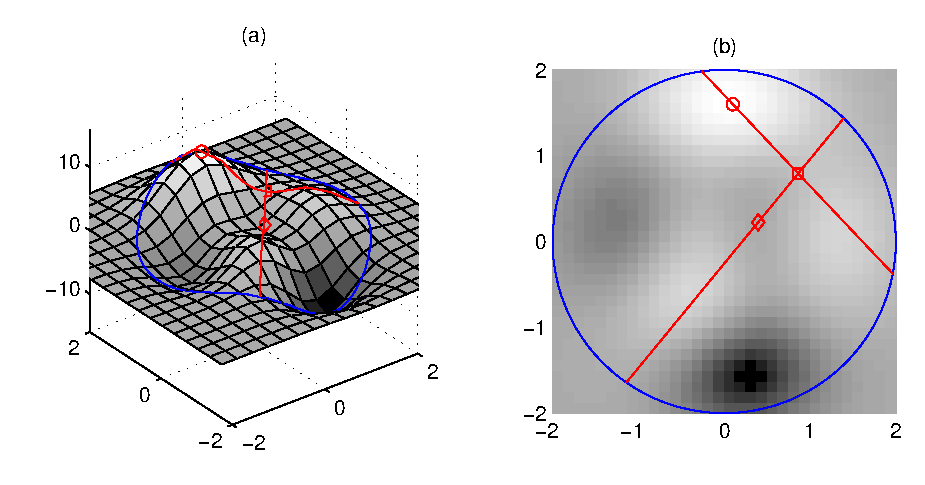
\includegraphics{figures/descent.epsg}
\end{center}
\begin{capt}{Schematic representation of gradient descent.}
Points within the circle are in \calH, the height of the surface
the value of (\ref{eqn:theory:cost function}) at that point.  (a) is a
3D view, (b) is top view. Lines show line searches; markers
minimums.  We descend from $\circ$ through $\Box$ to $\Diamond$, where
the algorithm terminates due to a local minima.
\end{capt}
\label{fig:gradient descent}
\end{linefigure}

This statement is formalised in the following theorem.

\begin{theorem}[AdaBoost implements gradient descent]
The AdaBoost algorithm implements gradient descent over a cost functional
%
\begin{equation}
Q(F, \bfx, y) = \exp \{-y F(\bfx) \}
\end{equation}
%
\proof We outline a skeleton, ignoring initial conditions and the
stopping conditions.  We will show that, given a state at iteration
$t$, then boosting and gradient descent produce identical states at
iteration $t+1$.

Once we have chosen $f_{t+1}$ using weighted empirical risk
minimisation, we need to choose $w_{t+1}$.  This is chosen to minimise
the cost functional along the line given by the direction $f_{t+1}$.
We can write the value of this cost functional as
%
\begin{equation}
C = \sum_{i=1}^{m} c \left( y_i F_t(\bfx_i) + y_i w_{t+1}
f_{t+1}(\bfx_i) \right)
\end{equation}
%
Substituting in $c(F(\cdot)) = e^{-yF(\cdot)}$, we obtain
%
\begin{equation}
C = \sum_{i=1}^{m} \exp \left\{ y_i F_t(\bfx_i) + y_i w_{t+1}
f_{t+1}(\bfx_i) \right\}
\end{equation}
%
Now we need to differentiate this expression with respect to
$w_{t+1}$.   This task is simplified considerably by noting that only
the second half of the exponential term is variable with $w_{t+1}$.
The result is that
%
\begin{eqnarray}{ll}
\label{eqn:differentiate}
\frac{\partial C}{\partial w_{t+1}} &
= & \sum_{i=1}^{m} \frac{\partial}{\partial w_{t+1}}
\exp \left\{ y_i F_t(\bfx_i) + y_i w_{t+1}
f_{t+1}(\bfx_i) \right\} \nonumber \\
& = & \sum_{i=1}^{m} y_i \exp \left\{ y_i F_t(\bfx_i) + y_i w_{t+1}
f_{t+1}(\bfx_i) \right\} 
\end{eqnarray}
%
From this result, we make several simplifications.  Noting that
%
\begin{equation}
y_i f_{t+1}(\bfx_i) = \left\{ 
	\begin{array}{ll}
	1 &	\qquad \mbox{if $y_i = f_{t+1}(\bfx_i)$} \\
	-1 &	\qquad \mbox{if $y_i \neq f_{t+1}(\bfx_i)$}
	\end{array}
\right.
\end{equation}
%
and that $w_{i | t} = k \exp \{ -y_i F_t(x_i) \}$ where $k$ is some
constant, we can recast (\ref{eqn:differentiate}) into the form
%
\begin{equation}
\underbrace{
	\frac{\sum_{i : y_i = f_{t+1}(\bfx_i)} w_{i|t}}
	     {\sum_{i : y_i \neq f_{t+1}(\bfx_i)} w_{i|t}}
}_{\epsilon_t}
= \exp \left\{ 2 \alpha \right\} 
\end{equation}
%
from which it is a simple transformation to obtain
(\ref{eqn:theory:bt}).  Thus, the state at iteration $t+1$ is
equivalent to boosting; thus boosting implements gradient descent.
\end{theorem}

The cost functional $c(\alpha) = e^{-\alpha}$ is an approximation to
the misclassification risk (\ref{eqn:misclassification risk}) that is
differentiable at all points and leads to a closed-form solution for
the step size.  It is plotted in figure \ref{fig:cost functional
approximation}.  Other approximations have been used; see Mason
et. al. \cite{Mason99} for details.

\begin{linefigure}
\begin{center}
\includegraphics{figures/cost_approx.epsg}
\end{center}
\begin{capt}{Approximation to the misclassification risk function}
The misclassification risk is plotted in the dotted line, with the
AdaBoost approximation plotted in the solid line.  It is clear that
the effect of this cost function will be to maximise the margins of
the samples.
\end{capt}
\label{fig:cost functional}
\end{linefigure}

\subsection{Summary}

In this section, we have shown that the AdaBoost algorithm implements
gradient descent.  There are four aspects of the gradient descent
problem that need to be specified:
%
\begin{enumerate}
\item	What is our universal set? (AdaBoost: $\co(\calH)$)
\item	What is our inner product? (AdaBoost: equation (\ref{eqn:inner
	product definition}))
\item	What is our cost function? (AdaBoost: $c(\alpha) =
	e^{-\alpha}$)
\item	How do we choose a step size? (AdaBoost: line search).
\end{enumerate}
%
In chapter \ref{chapter:development} we will consider changing some of
these to implement algorithms with desirable properties.

\section{AdaBoost and Boosting algorithms}

Until this point we have only considered the AdaBoost algorithm.  We
now extend our scope to other AdaBoost-like algorithms.  These
algorithms are termed ``boosting algorithms''.

There has recently been some debate over what constitutes a ``boosting
algorithm''; see for example Duffy and Helmbold \cite{Duffy99} who
adopt quite a restrictive definition.  In this thesis, we take a very
broad definition:

\begin{definition}[A boosting algorithm]
Any learning machine that constructs a hypothesis that is a linear
combination of base hypotheses by leveraging another learning machine
in an interative manner is a boosting algorithm.
\end{definition}

In particular, we don't require that the training error be guaranteed
to reach zero.  All algorithms considered in this thesis are,
according to definition \ref{def:boosting}, boosting algorithms.


\section{Properties of the AdaBoost and boosting algorithms}

We have covered the \emph{form} of the AdaBoost algorithm quite
extensively.  We now cover the \emph{function} of the algorithm, so
that we have a basis for comparison.

\subsection{Convergence properties}

This theorem provides two results.  The first, applicable to any
algorithm that implements gradient descent, shows that under certain
conditions on the cost function and step sizes the 
e main result of this section is a theorem that the empirical risk
(training error) of boosting will converge to zero if the algorithm is
trained for long enough.

\begin{theorem}[Boosting reaches zero training error]
Given a weaklearner $\mathcal{L}$ and a training set $S$,
then either:
\begin{enumerate}
\item	The boosting algorithm will terminate; or
\item	There exists an iteration $t_{zero}$ such that for all $t \geq
	t_{zero}$ the training error $\epsilon_t = 0$.
\end{enumerate}

\proof If for any training iteration $t$ we have $\epsilon_t \geq 1/2$
then the boosting algorithm will terminate.  Assuming that this is not the
case, let us look at $\|b\|$.  As $t \rightarrow \infty$, $\|b\|
\rightarrow \infty$.  Thus, taking the normalised hypotheses $\bar{h}_i
= b_i \frac{h}{\sum b}$ we obtain
\[
C(F_{t+1}) = \sum_{i=1}^{m} \exp\left\{ -y_i b_i h_i(x_i)
\right\}^{\|b\|}
\]
Now, we know from theorem (number?) that the boosting algorithm will
always find the global minimum of the cost function.  Since all $b_i >
0$, this is achieved when all training examples are classified
correctly...

Need a lot more work on this proof.  Do I want to show that since it
gets steeper and steeper, the cost of a negative sample gets too
large?  I don't think that the way I am doing it is going to work,
really.  I need to show that because
\begin{itemize}
\item	The weights for wrong samples are increasing exponentially,
	and
\item	The power that the cost function is raised to makes the wrong
	margin get worse and worse,
\end{itemize}
then the thingy gets minimised...

I need to bring the training error < 1/2 into it somewhere.  I think
that I can show that if
\begin{itemize}
\item	$\|b\|$ increases without bound; and
\item	$\epsilon_t$ is always < 1/2, then
\end{itemize}
I don't know!

\end{theorem}



\subsection{AdaBoost maximises the minimum margin}

This section introduces several theorems which together show that
AdaBoost chooses the linear combination that maximises the minimum
margin over its training samples.

\begin{theorem}[AdaBoost maximises the minimum margin]
Given a particular learning algorithm $F$ and a training
set $S$, define the minimum margin as
\[
m_{\min} = min_{\{x,y\} \in S} y_i F(x_i)
\]
Then the boosting algorithm will converge as $t \rightarrow \infty$ to
the solution which maximised the minimum margin.

\proof For boosting we can write $F_t = b_1 f_1 + \cdots + b_t f_t$.
Then defining our \emph{normalised hypotheses} $\bar{f}_i$ as
\[
\bar{f} = \frac{b_i f_i}{\|b\|}
\]
such that $\hat{F}_t = \bar{f}_1 + \cdots + \bar{f}_t$, we can write
our cost function (reference?) as 
\[
C(b, S) = \sum_{i=1}^{m} \exp\{-y_i \bar{F}_t(x_i)\}^{\|b\|}
\]
We already know from the gradient descent theory (reference?) that we
are trying to minimise the cost function.  Now as $\|b\| \rightarrow
\infty$ (from the previous theorem) the largest value of $\exp\{-y_i
\bar{F}_t(x_i)\}$ will dominate, and so $C(b, S) \rightarrow exp\{\max
-y_i \bar{F}_t(x_i)\}$.  Thus, by minimising $C(b, S)$, we are making
$\min y_i \bar{F}_t(x_i)$ as large as possible; that is we are
maximising the minimum margin.
\end{theorem}


\subsection{Equivalences of AdaBoost}

In this section we state two results that show scale independence of
the AdaBoost algorithm.

\begin{theorem}
The hypothesis returned by the AdaBoost is independent of a 
scaling of the $b$ values.  In particular, for all $k > 0$, the
scaled hypothesis $kF$ is equivalent to the unscaled hypothesis $F$.

\proof This follows from the fact that the sign function is
independent of a scaling of the $b$ values.
\end{theorem}




* Guaranteed convergence to zero training error

  * It modifies the weights at each iteration so the previous had
    $\epsilon_t = 1/2$

  * So we must keep on getting better

  * So we must converge

* Scale invariance

  * The sign makes it not matter

  * If we multiply $F_t$ by $k$ to get $F*_t$, then we get $b*_{t+1} = 1/k
    b_{t+1}$

* Converges to the solution that has the minimum margin
	
\subsection{Convergence of boosting}




\subsection{Size of $b$}

The following theorem shows that the total weight of the boosting
algorithm is unbounded as the number of iterations increases.  It is
used to prove results on the minimum margin and final training error
of boosting.

\begin{theorem}
The size of the $b$ weight vector, $\|b\| \rightarrow \infty$
as $t \rightarrow \infty$ (assuming the boosting algorithm doesn't
terminate).

\proof ?
\end{theorem}


\subsection{Minimum margin}

The following proof shows that the solution that AdaBoost converges to
is the one that maximises the minimum margin on the training samples.



We denote this equivalence by writing
\[
kF \equiv F
\]


\subsection{Scale invariance of AdaBoost}

The following theorem takes the previous result one step further,
showing that is AdaBoost is given a scaled hypothesis $kF$ instead of
$F$, it will choose a $b$ value that is also scaled by the same
amount.

this is not true... look at Gunnar's notes again

\begin{theorem}
Assume a strong hypothesis $F_t(\cdot) = b_1 f_1(\cdot) + \cdots + b_m
f_m(\cdot)$.  Denote the training action of the AdaBoost algorithm as
$F_t(\cdot) \Rightarrow F_{t+1}(\cdot) = F_t(\cdot) +
b_{t+1}f_{t+1}(\cdot)$.  If
\[
	F_t(\cdot) \Rightarrow F_t(\cdot) + b_{t+1}f_{t+1}(\cdot)
\]
then
\[
	kF_t(\cdot) \Rightarrow k\left( F_t(\cdot) +
	b_{t+1}f_{t+1}(\cdot) \right)
\]
and thus
\[
	kF_{t+1} \equiv F_{t+1}
\]

\proof We show that the minimum of the cost function occurs at
$kb_{t+1}$ instead of $b_{t+1}$.
\end{theorem}



These are from \cite{Ratsch98}:

\begin{theorem}[Weight update of AdaBoost (Schapire \cite{Schapire97})]
The weights $w_{i|t}$ in the $t$-th iteration are chosen such that the
previous hypothesis has exactly a weighted training error $\epsilon$
of $1/2$.
\end{theorem}

\subsection{Summary}


\section{Performance bounds for Boosting}

The following theorem appears in Schapire et. al \cite{Schapire97}.

\begin{theorem}[Performance bound for boosting ($p$=1)]

There is a constant $c$ such that a hypothesis $F$ generated by the
AdaBoost algorithm, from a base class $\calH$ with VC dimension $d$,
with probability at least $1 - \delta$ over $m$ independent training
samples
\begin{equation}
R(f) \leq R_{\emp}^{\gamma}(f) + \sqrt{\frac{c}{m} \left[ \frac{d
\ln^2 (m/d)}{\gamma^2} + \ln(1/\gamma) \right] }
\end{equation}
\end{theorem}


\subsection{Summary}

\section{Overfitting}

History of overfitting: looked like it didn't, then turned out to
for high noise or lots of iterations.

Explantion: maximising the minimum margin, thus the noisy points keep
on getting wronger.

This is why having an algorithm not ``maximising the minimum margin''
is not necessarily a bad thing... talk about DOOM II, deliberately
sacrafices minimum margin, gets better performance in some cases.
Mason et al \cite{Mason99}.

\section{Normed boosting algorithms}

Already been looked at by Mason et al \cite{Mason99a}, for $p=1$ and
$p=2$.  Different convergence results; converges to point in gradient
space where slope = 0 (surprise surprise); show how this does not
necessarily mean that training error is zero (because sum of
$b$ is now bounded, we don't get exponential fast decreasing to zero
of training error).

Describe the key differences between normed and unnormed:
\begin{itemize}
\item	Normed: renormalise after each step; unnormed: don't
\item	Normed: doesn't go to zero training error
\end{itemize}

Again, make the point that just because it doesn't minimise margins
doesn't mean that it's not going to work well --> give an argument why
it could work better (because not maximising minimum margin)


\section{Chapter summary}





\part{Theoretical development}
% pboosting.tex
% Jeremy Barnes, 22/9/1999
% $Id$

\chapter{$p$-boosting}

This chapter describes the concepts behind and a theoretical
justification of \emph{$p$-boosting}, a generalisation of the boosting
algorithm.  The treatment is somewhat abstract; further chapters will
be more concrete as practical issues are considered.

\section{$p$-convex hulls}

\section{$p$-boosting}

\section{Theoretical justification}



% development.tex
% Jeremy Barnes, 1999
% $Id$

\chapter{Development of algorithms}

\section{Scale invariance}

The boosting algorithm is sensitive only to the relative magnitude of
the classifier weights $b_i$, not to the absolute magnitude.

To see this, consider the linear combination of weights
%
\begin{equation}
y = \sign(F(\bfx)) = \sign(b_1 f_1(\bfx) + b_2 f_2(\bfx) + \cdots +
b_T f_T(\bfx)
\end{equation}
%
Now as
%
\begin{equation}
\sign(\alpha x) = \sign(x) \qquad \qquad \mbox{for $\alpha \neq 0$}
\end{equation}
%
a linear combination that is scaled by an $\alpha \neq 0$
%
\begin{equation}
y = \sign(F(\bfx)) = \sign(\alpha b_1 f_1(\bfx) + \alpha b_2 f_2(\bfx)
+ \cdots + \alpha b_T f_T(\bfx)
\end{equation}
%
is exactly the same as before.

For this reason, normalising of the weight vector is unnecessary.  It
also means that normalising to \emph{any} norm is equivalent to any
other norm; in particular, we will get equivalent behaviour by
normalising in a $p$-norm as we will in a $1$-norm.

\section{Refinement of gradient descent}

Once we have chosen $f_{t+1}$, we need to choose $w_{t+1}$.  This is
chosen to minimise the cost functional along the line given by the
direction $f_{t+1}$.  We can write the value of this cost functional
as
%
\begin{equation}
C = \sum_{i=1}^{m} c \left( y_i F_t(\bfx_i) + y_i w_{t+1}
f_{t+1}(\bfx_i) \right)
\end{equation}
Substituting in $c(f(x)) = e^{-yf(x)}$, we obtain
%
\begin{equation}
C = \sum_{i=1}^{m} \exp \left\{ y_i F_t(\bfx_i) + y_i w_{t+1}
f_{t+1}(\bfx_i) \right\}
\end{equation}
%
Now we need to differentiate this expression with respect to
$w_{t+1}$.   This task is simplified considerably by noting that only
the second half of the exponential term is variable with $w_{t+1}$.
The result is that
%
\begin{eqnarray}{ll}
\frac{\partial C}{\partial w_{t+1}} &
= & \sum_{i=1}^{m} \frac{\partial}{\partial w_{t+1}}
\exp \left\{ y_i F_t(\bfx_i) + y_i w_{t+1}
f_{t+1}(\bfx_i) \right\} \nonumber \\
& = & \sum_{i=1}^{m} y_i \exp \left\{ y_i F_t(\bfx_i) + y_i w_{t+1}
f_{t+1}(\bfx_i) \right\} 
\end{eqnarray}





\part{Testing}
% method.tex
% Jeremy Barnes, 22/9/1999
% $Id$

% Method baby...

\chapter{Experiments}
\label{chapter:method}

Extensive simulations of the $p$-boosting algorithms and AdaBoost were
run on a microcomputer in order to compare their performance, both
with the baseline AdaBoost algorithm, and with the theory developed in
previous chapters.  This chapter describes the experimental setup
(including a brief description of the software developed) and the
testing methodology to a level of detail sufficient to repeat the
experiments.

\section{Experimental setup}

In this section a summary of the equipment and computer software used
to perform the experiments is given.  The full source code, datasets
and test results are available on the CD-ROM attached inside the back
cover of this thesis.  Appendix \ref{appendix:cdrom} describes the
contents of this CD-ROM in more detail; appendix
\ref{appendix:datasets} the datasets; and appendix
\ref{appendix:software} the computer software.

\subsection{Hardware}

The simulations were run on three microcomputers.  The first was a
400MHz Celeron system with 256MB of memory, running RedHat Linux
version 6.0 and \MATLAB\ version 5.3.0.10183 (Release 11).  The second
was a 300MHz Celeron system with 128MB of memory, running RedHat Linux
version 5.2 and the same version of \MATLAB.  The third was a 233MHz
Cyrix M3 machine with 64MB of memory running Windows 95 version
4.00.1111 and \MATLAB\ version 5.0.0.4073 (Student version).

\subsection{Software}

Although an incidental part of the project, the software package that
was developed in order to perform the simulations is a significant
piece of work in its own right.  It was written from scratch to
allow an accessible and efficient entry into the project area--which
was not available at the commencement of the project.  In particular,
it includes many functions that allow visualisation of the algorithms.
Use of this package will significantly lower the difficulty of
beginning similar research or extending the ideas developed in this
project.

The software was written as a \MATLAB\ toolbox.  Two weak learning
algorithms (decision stumps and CART), several versions of the
Boosting algorithm (including all mentioned in this thesis), an
implementation of a Neural Network algorithm, an automated test
harness, and assorted analysis and visualisation functions are
included.  What follows is a brief description of the design and
implementation of the software package as a whole.  Individual
components are covered in appendix \ref{appendix:software}.

\subsection{Optimisation and numerical issues}

The code was profiled extensively using \MATLAB's inbuilt profiler,
and efficient algorithms selected for the frequently executed
sections.  Tight sections of code, and certain data and code
structures (for example, {\tt for} loops), which are inefficient under
\MATLAB, were recoded in \C\ to improve speed.  (Details of how
to interface this code were obtained from \cite{MathWorks96} and
\cite{MathWorks96a}.) As each function was optimised, its output was
compared with that of the un-optimised version to ensure equivalence
of the two versions of code.  The net effect of these optimisations
was that simulations which would have required several years to run as
initially coded were able to be run in a matter of days.

Minimising numerical errors was a major design goal.  Several sections
of code incorporate safeguards (such as periodic full recalculations
in loops that are optimised incremental calculations) to minimise the
effect of numerical errors.  In addition, 64 bit IEEE double precision
floating point numbers are used exclusively.

In total, the source code was 270KB in size, comprising 235KB of
\MATLAB\ code and 35KB of \C\ code.  There are approximately 10000
lines in 191 \MATLAB\ {\tt .m} files and 1500 lines in 6 \C\ source
files.  All source code was maintained under the {\tt CVS} version
control system.

\section{Datasets}

A total of seven datasets were used in the experiments.  Four
(\ds{ring0}, \ds{ring10}, \ds{ring20} and \ds{ring30}) were
synthetic datasets, randomly generated from a known distribution with
noise added artificially.  Two other datasets (\ds{sonar} and
\ds{wpbc}%
\footnote{Wisconsin Prognostic Breast Cancer.}
) were obtained from the UCI repository \cite{UCI}, and the
final dataset (\ds{acacia}) was ecological data used in a PhD thesis
\cite{Payne97}.  A summary of the features of each dataset appears in table
\ref{tbl:datasets} (Appendix \ref{appendix:datasets} describes the
datasets in more detail.)  This group was selected to cover a broad
range of situations:  the four \ds{ring} datasets allow the effect of
noise to be isolated and contain a very high sample-to-attribute
ratio;  the \ds{sonar} dataset is low-noise (generated from precise
measurements ) but contains a low sample-to-attribute ratio; and the
\ds{wpbc} and \ds{acacia} datasets are examples of difficult and very
difficult%
\footnote{Difficult and very difficult in that previous applications
of machine learning algorithms to these datasets produce indifferent
to poor results.}%
real-world data.

\begin{table}
\begin{center}
\begin{tabular}{l c c r r r r}\hline
{\bf Dataset} & $\calI$ & $\calO$ & {\bf Artificial noise} & {\bf
Size} & {\bf Training samples} & {\bf Test samples} \\
\hline \hline
\ds{ring0} & $[0,1]^2$ & $\{\pm 1\}$ & 0\% & $\infty$ & 50 & 5000 \\
\ds{ring10} & $[0,1]^2$ & $\{\pm 1\}$ & 10\% & $\infty$ & 50 & 5000 \\
\ds{ring20} & $[0,1]^2$ & $\{\pm 1\}$ & 20\% & $\infty$ & 50 & 5000 \\
\ds{ring30} & $[0,1]^2$ & $\{\pm 1\}$ & 30\% & $\infty$ & 50 & 5000 \\
\hline
\ds{sonar} & $[0,1]^{60}$ & $\{\pm 1\}$ & 0\% & 208 & 70 & 138 \\
\ds{wpbc} & $\subset \bbR^{33}$ & $\{\pm 1\}$ & 0\% & 194 & 97 & 97 \\
\ds{acacia} & $\subset \bbR^{16}$ & $\{\pm 1\}$ & 0\% & 204 & 102 & 102 \\
\hline
\end{tabular}

{\small Note that samples with missing attribute values were excluded
from each dataset.}
\end{center}
\caption{Summary of dataset attributes}
\label{tbl:datasets}
\end{table}

\section{Testing}

In this section we detail the aims of the experiments, the procedure
that was followed, and how the results were summarised and analysed.

\subsection{Aims}
The aims of the experiments were four-fold:
%
\begin{enumerate}
\item	To test the generalisation performance of the $p$-boosting
	algorithms, and how this performance compares with the
	that of AdaBoost.  It was expected that the $p$-boosting
	algorithms would outperform AdaBoost on noisy datasets.

\item	To verify that the qualitative behaviour (and quantitative
	behaviour wherever possible) of the $p$-boosting algorithms
	matched the theory developed in chapters \ref{chapter:slt},
	\ref{chapter:boosting} and \ref{chapter:pboosting}:
	%	
	\begin{itemize}
	\item	The $p$ parameter controls the capacity of the
		function class.  Thus, a generalisation error vs $p$
		plot should have a minimum at some optimal value
		$p^{\ast}$ (figure \ref{fig:optimal p value}).
	\item	The confidence interval in theorem \ref{thm:p convex
		generalisation} decreases as $p \rightarrow 0$.  As a
		result, the true risk (test error) and empirical risk 
		(training error) curves should match closely as $p
		\rightarrow 0$.
	\end{itemize}
	
\item	To verify that the algorithms were operating as designed.
	It was expected that a distribution of classifier weights
	would show that most of the weight is given to fewer and fewer
	classifiers for low $p$ values.

\item	To test the efficiency of the algorithms as compared to
	AdaBoost.  An algorithm that generates a slightly better
	hypothesis but takes much longer to train may not be
	considered an improvement in some applications.
\end{enumerate}

\subsection{Method}

A total of 31 tests were run, as detailed in table
\ref{tbl:experiments}.  Each test involved training a particular
algorithm on a dataset (up to a maximum of \emph{Iterations} training
iterations).  The test was repeated for \emph{Trials} independent
trials, each time with a newly generated (\ds{ring*}) or randomly
permuted and partitioned (\ds{sonar}, \ds{wpbc}, \ds{acacia})
test and training dataset%
\footnote{Note that noise was added to the training \ds{ring*}
datasets but \emph{not} the test \ds{ring*} datasets.}%
, and this whole procedure repeated for each $p$ value.

\newcommand{\allp}{$\frac{1}{2} \leq p \leq 2; 10p \in \bbN$}
\newcommand{\lowp}{$\frac{1}{2} \leq p \leq 1; 10p \in \bbN$}
\begin{table}
\begin{center}
\begin{tabular}{r l l r r c}\hline
{\bf Number} & {\bf Algorithm} & {\bf Dataset} & {\bf Trials} &
{\bf Iterations} & {\bf $p$ values} \\
\hline\hline
1-4  & AdaBoost & \ds{ring*}   & 100 &  1000 & - \\
5    & AdaBoost & \ds{sonar}   &  30 &  1000 & - \\
6    & AdaBoost & \ds{wpbc}    &  50 & 10000 & - \\
7    & AdaBoost & \ds{acacia}  &  50 & 10000 & - \\
\hline
8-11 & Na\"{\i}ve & \ds{ring*} &  50 &  1000 & \allp \\
12   & Na\"{\i}ve & \ds{sonar} &  30 &  1000 & \allp \\
\hline
13-16 & Strict & \ds{ring*}    &  30 &  1000 & \allp \\
17    & Strict & \ds{sonar}    &  50 & 10000 & \allp \\
18    & Strict & \ds{wpbc}     &  20 &  5000 & \allp \\
19    & Strict & \ds{acacia}   &  20 & 10000 & \allp \\
\hline
21-24 & Sloppy & \ds{ring*}    &  30 &  1000 & \allp \\
25-28 & Sloppy & \ds{ring*}    &  30 & 10000 & \lowp \\
29    & Sloppy & \ds{sonar}    &  50 & 10000 & \allp \\
30    & Sloppy & \ds{wpbc}     &  20 &  5000 & \allp \\
31    & Sloppy & \ds{acacia}   &  20 & 10000 & \allp \\
\hline  
\end{tabular}

\small{The weak learning algorithm is always \emph{decision stumps}.}
\end{center}
\caption{Summary of experiments conducted}
\label{tbl:experiments}
\end{table}

The following data was recorded for each trial:
%
\begin{itemize}
\item	All test parameters;
\item	Test and training datasets;
\item	Training and test error (unweighted) at each iteration;
\item	Margins of the training samples at both the iteration with the
	minimum \emph{test} error and the final iteration;
\item	Classifier weights at the final iteration.
\end{itemize}


\subsection{Analysis}

More than two gigabytes of data was generated in the course of
testing.  This data was summarised across all trials for each (test,
p-value) combination, and a summary file created.  The summary file
contained the following information:
%
\begin{itemize}
\item	The mean and standard deviation of test and training error
	curves at each iteration;
\item	The number of trials that had not aborted before each
	iteration (recall that the algorithms would abort if the
	training error exceeded $\frac{1}{2}$, fell below $0$, or if
	the cost function was strictly increasing); 
\item	The value of the best (lowest) test error
	$\underset{X_T}{R_{\emp}}$ for each trial, and the number of
	training iterations after which this best error value
	occurred;
\end{itemize}
%
Each of the $p$-boosting algorithms had further statistics produced
for each $p$ value.  These statistics were:
%
\begin{itemize}
\item	The mean and standard deviation of the best test error at each
	$p$ value, over all trials;
\item	The mean and standard deviation of the number of training
	iterations the best error was produced at, over all trials.
\end{itemize}

For each of the $p$-boosting algorithms, a crude form of structural
risk minimisation (see section \ref{sec:theoretical overfitting}) was
then performed, by selecting the $p$ value with the \emph{lowest mean
best test error} to be $p^{\ast}$ (see figure \ref{fig:effect of p} on
page \pageref{fig:effect of p}).  This is the $p$ value that is used 
whenever comparisons of the performance of algorithms are made (it
makes little sense to compare anything but the \emph{best}
performance!)  The entire analysis described above was repeated for
each dataset.






% results.tex
% Jeremy Barnes, 22/9/1999
% $Id$

\chapter{Results and discussion}
\label{chapter:results}

\section{Generalisation performance}

\begin{linefigure}
\begin{center}
\includegraphics{figures/test_err_summary.epsg}
\end{center}
\begin{capt}{Comparison of AdaBoost and $p$-boosting test
generalisation performance}{fig:test err summary}
Each part plots the \emph{average test error value} of AdaBoost
against the \emph{average test error value} of the specified algorithm
\emph{at the point of minimum training error}.  The shape of the
marker indicates the dataset: $\bullet$ \ds{ring0}, $\times$
\ds{ring10}, $\circ$ \ds{ring20}, $\ast$ \ds{ring30}, $\Box$
\ds{sonar}, $\bigtriangleup$ \ds{wpbc}, $\Diamond$ \ds{acacia}.  The
bars indicate one standard deviation each side of each datapoint.

Points above the line indicate that the algorithm generalises performs
better than AdaBoost on that particular dataset.
\end{capt}
\end{linefigure}


\section{Effect of $p$ value on generalisation performance}

\begin{linefigure}
\begin{center}
\includegraphics{figures/effect_of_p.epsg}
\end{center}
\begin{capt}{Effect of $p$ on generalisation error}{fig:effect of p}
Average test error of each algorithm: AdaBoost (thick line), strict
(thin solid), sloppy (dash-dot) and na\"{\i}ve (dotted) is shown for
each dataset.  The bullets $\bullet$ indicate the best value of $p$
which is used in figure \ref{fig:test err summary}.
\end{capt}
\end{linefigure}

\section{Training time}

Figure \ref{fig:test iter summary} details how the training times
compare with AdaBoost.  We can see that the...

\begin{linefigure}
\begin{center}
\includegraphics{figures/test_iter_summary.epsg}
\end{center}
\begin{capt}{Comparison of AdaBoost and $p$-boosting training
times}{fig:test iter summary} 
Both axes measure numbers of iterations.  The $y$ axis measures the
average number of iterations required for AdaBoost to reach the
minimum of the test error; the $y$ axis is the same statistic for the
$p$-boosting variant \emph{at the optimal value of $p$}.  Points above
the line indicate that AdaBoost requires more iterations to train than
the other algorithm.  Marker symbols indicate datasets; see figure
\ref{fig:test err summary} for a legend.
\end{capt}
\end{linefigure}

\subsection{Possible remedy to inefficient training}

It may be possible to accelerate the training of the sloppy algorithm
by choosing a more aggressive cost function.  We modify the cost
function to be of the form
%
\begin{equation}
c(\alpha) = e^{-\alpha t^\lambda}
\end{equation}
%
where $t$ is the iteration number, and $\lambda$ a constant parameter
that controls how accelerated the learning process should be.  This
cost function gets steeper as the number of iterations increases.
Insufficient time was available to perform experiments using this cost
function, however.


\section{Margin distributions}


\begin{linefigure}
\begin{center}
\includegraphics{figures/margin_distribution.epsg}
\end{center}
\begin{capt}{Margin distribution of algorithms}{fig:margin distribution}
\end{capt}
\end{linefigure}


\section{Other observations}

\subsection{AdaBoost}

\subsection{Naive $p$-boost}

..blah...

Thus, we observe that the actual distribution of \emph{classifier}
weights has little influence on the generalisation ability of the
AdaBoost algorithm, and therefore it is the \emph{sample} weights that
cause the success of the algorithm.  This phenomena has also been
observed by Breiman \cite{Breiman96}.



\part{Discussions}
% discussion.tex
% Jeremy Barnes, 6/10/1999
% $Id$

\chapter{Discussion}
\label{chapter:discussion}
% furtherwork.tex
% Jeremy Barnes, 21/9/1999
% $Id$

\chapter{Further work}

This chapter describes open questions and lines of enquiry that could
be pursued to continue this work.



% conclusion.tex
% Jeremy Barnes, 6/10/1999
% $Id$

\chapter{Conclusion}
\label{chapter:conclusion}

In this thesis we have considered variants of the AdaBoost machine
learning algorithm, with the desireable property of explicit capacity
control.  Capacity control is implemented by confining the class of
allowable combined hypotheses to lie on the $p$-convex hull of the
underlying hypotheses, and is adjustable via the $p$ parameter.

Theoretical results indicate that the performance of these adjustable
algorithms for the optimal $p$ value may be superior to AdaBoost,
especially in the presence of large amounts of label noise (where
AdaBoost is prone to overfitting).  The approximate and bounded-above
form of these theoretical results prevent stronger statements being
made.

Several variants of a ``$p$-boosting'' algorithm were developed.  The
first variant used a na\"{\i}ve approach, and its performance was not
significantly different from that of the AdaBoost algorithm.  The
second variant (``strict'') was confined strictly along the $p$-convex
hull at all times, but proved to be prone to early stopping for $p <
1$.  The third variant (``sloppy'') was less restricted during the
line search phase (searching along the same line as AdaBoost).

The strict algorithm performed poorly as compared to AdaBoost and the
sloppy algorithm, both in terms of generalisation performance and
training time.  It is hypothesised that the observed behaviour is a
result of the gradient descent optimisation not finding the global
minimum.  The sloppy algorithm performed well on noisy datasets, with
the shape of the capacity-vs-generalisation error curve matching the
theoretical prediction, and the generalisation error at the optimal
$p$ value significantly up to 25\% improved on AdaBoost.  However,
both the strict and the sloppy algorithms required approximately an
order of magnitude more training iterations than AdaBoost to reach the
optimal solution.  An accelerated version is proposed that may improve
on this situation.

In conclusion, the capacity controlled ``$p$-boosting'' algorithms
considered in this project have been shown to be an improvement on
AdaBoost in some situations.  More extensive testing is required
before further conclusions can be drawn.



\appendix

% Put it back to normal for the non-body parts of the thesis.
\renewcommand{\baselinestretch}{1.0}
% acronyms.tex
% Jeremy Barnes, 1999
% $Id$

\section*{Acronyms}

\begin{tabular}{l l l}

\bf{Acronym} & \bf{Meaning} & \bf{First introduced} \\ \hline \hline

SLT	& Statistical Learning Theory 	& section \ref{acr:slt} \\
ERM	& Empirical Risk Minimisation 	& section \ref{acr:erm} \\
SRM	& Structural Risk Mininmisation & section \ref{acr:srm} \\
VC dimension & Vapnik-Chervonenkis dimension & section \ref{acr:vcdim} \\
CART	& Classification And Regression Trees & section \ref{acr:cart} \\
\hline

\end{tabular}


% notation.tex
% Jeremy Barnes, 1999
% $Id$

\chapter{Notation and Acronyms}

\newcommand{\notationskip}{5mm}
\newcommand{\notspace}{\vspace{\notationskip}}

\section*{Notation}
\newcommand{\longexp}[1]{\parbox[t]{3in}{\raggedright #1}}
\begin{tabular}{l l c}
\bf{Symbols}		& \bf{Meaning}		& \bf{Section} \\
\hline \hline
$\bfx \in \calI$	& Sample
			& fig \ref{fig:supervised learning} \\

$y \in \calO$		& Label
			& " \\

$X = ((\bfx_1, y_1), \ldots))$
			& Labeled samples, length $m$ (training dataset)
			& \ref{sec:formulation} \\

\notspace
$\calI, \calO$		& Domain and range (usually $\{\pm 1\}$) of problem
			& \ref{sec:domain and range} \\
$h(\cdot) \in \calH : \calI \mapsto \calO$
			& A hypothesis (classifier)
			& \ref{sec:formulation} \\

$\calH$			& A set of possible hypotheses $h$
			& \ref{representation learning machines} \\

$f(\cdot) \in \calF : \calI \mapsto \bbR$
			& \longexp{A non-thresholded hypothesis; usually 
			  $h(\cdot) = \sign(f(\cdot))$}
			& \ref{sec:margin formulation} \\

$\calF$			& A set of possible hypotheses $f$ 
			  ($\calH = \sign(\calF)$)
			& " \\

\notspace
$\bbW : \calI^m \mapsto (\calI \mapsto \calO)$
 			& Learning machine ($\bbW(X) = h$)
			& " \\
$q = Q(\bfx, y, \hat{y})$
			& Loss function
			& \ref{sec:loss function} \\

$R(h)$			& True risk
			& \ref{sec:true risk} \\

$R_{\emp}(h)$		& Empirical risk
			& \ref{sec:empirical risk} \\

$R_{\emp}^w(h)$		& Weighted empirical risk (training error)
			& \ref{sec:weighted empirical risk} \\

\notspace
$R_{\emp}^{\gamma}(h)$	& Margin risk
			& \ref{sec:margin risk} \\

$\VCdim(\cdot)$		& VC dimension
			& \ref{sec:vcdim} \\

$\covert{\calX}{\epsilon}{d(\cdot, \cdot)}$ &
			\longexp{Covering number at scale $\epsilon$ of $\calX$
			using norm $d$ (usually $d_{\infty}$; assumed if not
			specified)}
			& \ref{sec:covering numbers} \\

$\covert{\calX}{\epsilon}{k}$ &
			\longexp{
			Uniform covering number of $\calX$ at scale $\epsilon$
			over length $k$}
			& " \\

\notspace
$\co_{p}(\calX)$, $\co(\calX)$
			& \longexp{$p$-convex hull of set $\calX$; $p=1$
			 assumed if not specified}
			& \ref{sec:p-convex} \\
$\bbB$, $\trainboost$	& AdaBoost, action of AdaBoost
			& \\
$F(\bfx)$, $H(\bfx)$	& \longexp{Boosting hypothesis, nonthresholded
			\& thresholded, $H(\cdot) = \sign(F(\cdot))$}
			& \\

$b_1, \ldots, b_t$	& AdaBoost classifier weights
			& \\

$w_1|_t, \ldots, w_m|_t$ & AdaBoost sample weights
			& \\

\hline
\end{tabular}
\par\par\noindent
A hat ($\hat{\ \ }$) means ``estimate''.  An asterisk ($\ \ ^{\ast}$) means
``optimal'' in some sense.


\section*{Acronyms}

\begin{tabular}{l l l}

\bf{Acronym} & \bf{Meaning} & \bf{First introduced} \\ \hline \hline

SLT	& Statistical Learning Theory 	& \ref{acr:slt} \\
ERM	& Empirical Risk Minimisation 	& \ref{acr:erm} \\
SRM	& Structural Risk Mininmisation & \ref{acr:srm} \\
VC dimension & Vapnik-Chervonenkis dimension & \ref{acr:vcdim} \\
\hline

\end{tabular}


\chapter{Implementation of learning algorithm}

% userguide.tex
% Jeremy Barnes, 21/9/1999
% $Id$

\providecommand{\emp}{\mathrm{emp}}
\providecommand{\calF}{\ensuremath{\mathcal{F}}}
\providecommand{\fat}{\ensuremath{\mathrm{fat}}}
\providecommand{\sign}{\ensuremath{\mathrm{sign}}}
\providecommand{\cop}{\ensuremath{\mathrm{co}_p}}
\providecommand{\co}{\ensuremath{\mathrm{co}}}
\providecommand{\bfx}{\ensuremath{\mathbf{x}}}
\providecommand{\bfy}{\ensuremath{\mathbf{y}}}
\providecommand{\bfyh}{\ensuremath{\hat{\mathbf{y}}}}
\providecommand{\calO}{\ensuremath{\mathcal{O}}}
\providecommand{\calI}{\ensuremath{\mathcal{I}}}
\providecommand{\calH}{\ensuremath{\mathcal{H}}}


\chapter{User's guide for machine learning library}

\section{Introduction}

\subsection{Class taxonomy}

\subsection{Common methods}

\subsection{Base classes}

\subsection{Category list}

\subsection{Dataset}

\subsection{Weak learner}

\section{Weaklearners}

\subsection{Decision stumps}

\subsection{CART}

\subsection{Neural Networks}

\section{Boosting algorithms}

\subsection{Boosting}

\subsection{P-boosting}

\section{Support routines}

\subsection{Visualisation}

\subsection{Data manipulation}


% progguide.tex
% Jeremy Barnes, 21/9/1999
% $Id$

\providecommand{\emp}{\mathrm{emp}}
\providecommand{\calF}{\ensuremath{\mathcal{F}}}
\providecommand{\fat}{\ensuremath{\mathrm{fat}}}
\providecommand{\sign}{\ensuremath{\mathrm{sign}}}
\providecommand{\cop}{\ensuremath{\mathrm{co}_p}}
\providecommand{\co}{\ensuremath{\mathrm{co}}}
\providecommand{\bfx}{\ensuremath{\mathbf{x}}}
\providecommand{\bfy}{\ensuremath{\mathbf{y}}}
\providecommand{\bfyh}{\ensuremath{\hat{\mathbf{y}}}}
\providecommand{\calO}{\ensuremath{\mathcal{O}}}
\providecommand{\calI}{\ensuremath{\mathcal{I}}}
\providecommand{\calH}{\ensuremath{\mathcal{H}}}


\chapter{Programmer's guide for machine learning library}

\section{Installation and compilation}

\section{Object oriented programming}

\section{Utilities}

\subsection{{\tt matlabscript}}



\chapter{Project proposal}
\label{chapter:proposal}

\begin{center}
{\Large DRAFT Honours Project Proposal:
Capacity Control in Boosting via an Adjustable  b Function
\footnote{This project was originally called, ``Aspects
of Statistical Learning Theory and Support Vector Machines''} \\
Jeremy Barnes \\
Supervisor: Dr Bob Williamson}
\end{center}

\section{Introduction}
The aim of this document is to provide some detail on the scope and
implementation of this honours project.  A brief background on the
project is given; followed by an explicit statement of the expected
outcomes; and a timeline.

\section{Background}
Boosting is a method used to improve the generalisation ability of a
"weak" learning algorithm.  It is implemented by generating many
instances of the algorithm, each trained on different data.  This data
is chosen such that examples which are commonly misclassified are
emphasised.  This forces the learning algorithm to work well with the
difficult data, and have better overall performance.  The output of
the boosting algorithm is a weighted combination of the outputs of the
weak learning algorithms (weighted by their performance).

Adjusting the capacity of a learning algorithm controls the size of
the set of possible generalisations.  It is important to control
capacity to avoid overfitting (fitting the noise rather than the
underlying function).  Although boosting is particularly good at
avoiding overfitting, implementing capacity control can improve the
performance of the boosted algorithm [ref] and avoid eventual
overfitting.

The $b$ function is used within the boosting algorithm.  It is
calculated for each instance of the weak learning algorithm, from the
learning error of the weak learning algorithm (the learning error is
the proportion of samples which are misclassified).  In the case of a
binary classification problem, it has the form
%
\begin{equation}
b_t = \log \frac{\epsilon_t}{1-\epsilon_t} \qquad (0 \leq \epsilon_t
\leq 1)
\end{equation}
%	
where $\epsilon_t$ is the learning error of weak learning algorithm  $t$.

	This function describes the ``worth'' of this instance of the weak
learning algorithm.  A plot is shown in figure 1.

\begin{figure}
\begin{center}
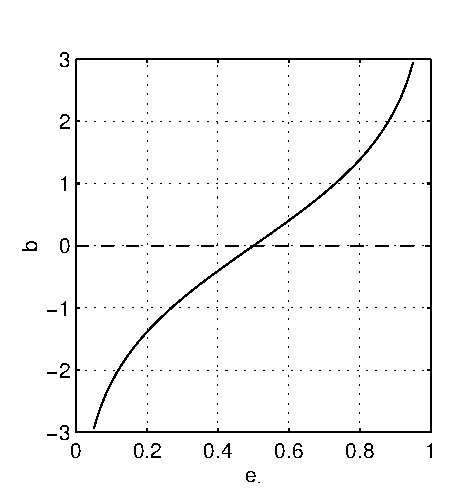
\includegraphics{figures/bfunc.eps}
\end{center}
\caption{The $b_t$ function versus error $\epsilon_t$}
\end{figure}
 
Weak learners with a value of $\epsilon_t$ around $1/2$ are worthless,
as random guessing performs just as well.  As $epsilon_t$ moves away
from $1/2$, the algorithms become more useful (and show an increase in
$b_t$ ).  Algorithms that approach $\epsilon_t \rightarrow \pm 1$ are
given a $b_t$  that approaches $\pm \infty$.

This project will investigate modifying the b function to become
\begin{equation}
b^{\prime}_t = \mathrm{sign}(b_t) |b_t|^{1/p}
\end{equation}
The new parameter p allows control over how aggressively weak learners
are penalised.  This should allow capacity control via adjustment of
this parameter.

\section{Outcomes}
The project will be successful if the following outcomes are attained:

\begin{itemize}
\item	Enough experimental evidence is gathered to gain an
	appreciation of the effect of the   parameter on the boosting
	algorithm.

\item	From this evidence, some guiding principles for improving the
	performance of the boosting algo-rithm using the   parameter
	are developed.

\item	Theoretical justification of these results is obtained.
\end{itemize}

In addition to these goals, it is hoped that progress in one or more of the following areas will be made:

\begin{itemize}
\item	Performance of the algorithm in problems with varying amounts
	of noise;

\item	Improved versions on the p-boosting algorithm using knowledge
	gained from the theory;

\item	Improving the computational efficiency of boosting using the
	p-boosting algorithm;

\item	Comparisons between p-boosting and other methods of capacity
	control in boosting;

\item	Extension of the results to include arbitrary classification
	problems;

\item	Extension of the results to include regression problems;

\item	Extension of the results to include other enhancements to the
	boosting algorithm, such as "soft margins" \cite{Ratsch98}.
\end{itemize}

In order to limit the project to a reasonable scope, initially the following constraints will be placed:

\begin{itemize}
\item	Only binary classification problems will be considered.

\item	Small datasets will be used.

\item	Simple weak learning algorithms will be used.
\end{itemize}


\section{Timeline}
This section includes a month-by-month description of what I intend to
complete on the project.  It is given in table \ref{table:timeline} on
page \pageref{table:timeline}.

\begin{table}
\begin{tabular}{r l}
\textbf{Month}		& \textbf{Tasks} \\ \hline \hline
December 1998		& Reading \\ \hline
January 1999		& Reading \\ \hline
February 		& Reading \\ \hline
March			& Writing project proposal \\
			& \textbf{19th Project proposal due} \\
			& Obtaining or writing code for experiments \\ \hline
April			& Writing, debugging code \\
			& 12th Code running, first test results \\
			& Obtaining datasets, running tests, refining
			  code  \\ \hline
May			& Running tests \\
			& Developing and testing hypotheses \\
			& Reading on theory \\
			& \textbf{31st First draft of "background"
			  section of thesis} \\ \hline
June			& Initial attempts at theoretical analysis \\
			& Running tests required for theoretical
			  verification \\
			& Attempting to reach closure on some aspects \\
			& \textbf{Exam period} \\ \hline
July			& Attempting to reach closure on some aspects \\
			& Writing progress report \\
			& \textbf{19th Progress report due} \\
			& Preparing for seminar \\
			& \textbf{26th Seminar} \\ \hline
August			& Final work on theory \\
			& Final experimental results to assist theory \\
			& \textbf{30th Sufficient work done to
			  complete thesis} \\ \hline
September		& Work on spin-off or extension aspects \\
			& Preparing for demonstration \\
			& \textbf{27th All experimental and
			  theoretical results obtained} \\
			& Writing thesis \\ \hline
October			& Writing thesis \\
			& \textbf{7th Draft thesis due} \\
			& Revising thesis \\
			& \textbf{27th Thesis due} \\
			& \textbf{28th Demonstration} \\
\hline
\end{tabular}
\caption{Project timeline}
\label{table:timeline}
\end{table}

\noindent\textbf{Notes:}

\begin{itemize}
\item 	I intend to work on the thesis gradually throughout the year,
	so that I do not need to write it all at the end.

\item	I have allowed 2-3 weeks to work on "extension" aspects of the
	problem that are interesting but not vital to a strong thesis.  It
	would not be a serious problem if none of this work can be included in
	the thesis.  These 2-3 weeks also give me some slack if things are not
	going as planned or if I become burnt out and need a break.
\end{itemize}



\backmatter

\bibliography{../Bibliography/biblio}
\bibliographystyle{plain}

\end{document}


